\documentclass{beamer}
\usepackage{tikz}
\usetikzlibrary{calc,arrows.meta,patterns}
\usepackage{xcolor}
\usepackage{multicol}
\usepackage{amsmath}

\title{Circles: Area, Squaring \& Pi}
\author{}
\date{}

\begin{document}

\frame{\titlepage}

%------------------------------------------------
% SLIDE 1: Retrieval + Squaring as a New Skill
%------------------------------------------------
\begin{frame}{Starter}

\begin{columns}

\column{0.35\textwidth}
\begin{center}
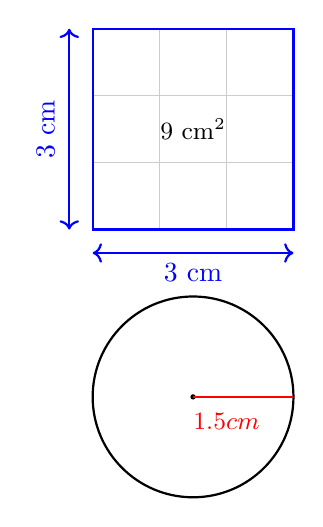
\begin{tikzpicture}[scale=0.85]
  % Grid of squares to illustrate squaring / area idea
  \draw[gray!40, thin] (0,0) grid (3,3);
  \draw[thick, blue] (0,0) rectangle (3,3);
  \draw[blue, thick, <->] (0,-0.35) -- (3,-0.35);
  \node[blue] at (1.5,-0.65) {$3$ cm};
  \draw[blue, thick, <->] (-0.35,0) -- (-0.35,3);
  \node[blue, rotate=90] at (-0.7,1.5) {$3$ cm};
  \node at (1.5,1.5) {\small $9$ cm$^2$};

  % Small circle below for context
  \draw[thick] (1.5,-2.5) circle (1.5cm);
  \fill (1.5,-2.5) circle (0.04);
  \draw[red, thick] (1.5,-2.5) -- ++(0:1.5);
  \node[red, below] at (2,-2.6) {\small $1.5cm$};
\end{tikzpicture}
\end{center}

\column{0.65\textwidth}
\small
\begin{enumerate}
  \begin{multicols}{2}
    \item $4 \times 4 = \ ?$
    \item $7 \times 7 = \ ?$
  \end{multicols}
  \begin{multicols}{2}
    \item $10^2 = \ ?$
    \item $3^2 = \ ?$
  \end{multicols}
  \item $2 \times 6$ and $6^2$ — are these the same? 
  \begin{multicols}{2}
  \item $3.14 \times 9 =$
  \item $3.14 \times 25=$
  \end{multicols}
\end{enumerate}
\vspace{-1em}
\begin{enumerate}
  \setcounter{enumi}{6}
  \item A circle has \textbf{diameter} $14$ cm. Find: \newline{} (a) the radius \newline{} (b) the circumference. ($\pi \approx 3.14$)
  \item A circle has \textbf{radius} $5$ cm. What is the circumference?
  \item The square has side $3$ cm and area $9$ cm$^2$. A circle has radius $1.5$ cm. Is the circle's area more or less than $9$ cm$^2$?
\end{enumerate}

\end{columns}
\end{frame}

%------------------------------------------------
% SLIDE 2: Retrieval + Radius vs Diameter + Squaring in Context
%------------------------------------------------
\begin{frame}{Starter}

\begin{columns}

\column{0.35\textwidth}
\begin{center}
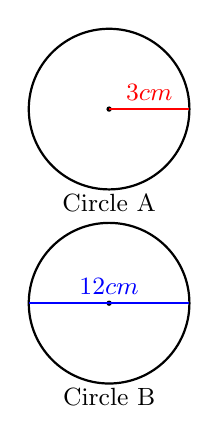
\begin{tikzpicture}[scale=0.85]

  % Circle A — radius labelled
  \draw[thick] (0,2.5) circle (1.2cm);
  \fill (0,2.5) circle (0.04);
  \draw[red, thick] (0,2.5) -- ++(0:1.2);
  \node[red] at (0.6, 2.75) {\small $3cm$};
  \node at (0, 1.1) {\small Circle A};

  % Circle B — diameter labelled
  \draw[thick] (0,-0.4) circle (1.2cm);
  \fill (0,-0.4) circle (0.04);
  \draw[blue, thick] (-1.2,-0.4) -- (1.2,-0.4);
  \node[blue] at (0,-0.15) {\small $12cm$};
  \node at (0,-1.8) {\small Circle B};

\end{tikzpicture}
\end{center}

\column{0.65\textwidth}
\small
\begin{enumerate}
  \begin{multicols}{2}
    \item Halve $12$ cm
    \item Halve $9.4$ cm
  \end{multicols}
  \begin{multicols}{2}
    \item $6^2 = \ ?$
    \item $1.5^2 = \ ?$
  \item $3 \times 4^2=$
  \item True or false? $\pi \times (2r) = 2 \times \pi \times r$
  \end{multicols}
\end{enumerate}
\vspace{-2em}
\begin{enumerate}
  \setcounter{enumi}{6}
  \item Consider circle A \newline{} (a) What is the circumference? \newline{} (b) What is the area?
  \item Consider circle B \newline{} (a) What is the circumference? \newline{} (b) What is the area?
  \item Is the ratio of the cirumferences of circle's A and B the same as the ratio of the areas?
\end{enumerate}

\end{columns}
\end{frame}

%------------------------------------------------
% SLIDE 3: Retrieval + Area Intuition + First Explicit Area
%------------------------------------------------
\begin{frame}{Starter}

\vspace{-1em}

\begin{columns}

\column{0.35\textwidth}
\begin{center}
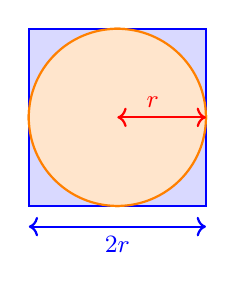
\begin{tikzpicture}[scale=0.75]
  \draw[thick, blue] (0,0) rectangle (3,3);
  \draw[thick, orange] (1.5,1.5) circle (1.5cm);
  \fill (1.5,1.5) circle (0.04);

  % Shade corners to show wasted space
  \begin{scope}
    \clip (0,0) rectangle (3,3);
    \fill[blue!15] (0,0) rectangle (3,3);
    \fill[orange!20] (1.5,1.5) circle (1.5cm);
  \end{scope}
  \draw[thick, blue] (0,0) rectangle (3,3);
  \draw[thick, orange] (1.5,1.5) circle (1.5cm);

  \draw[red, thick, <->] (1.5,1.5) -- ++(0:1.5);
  \node[red] at (2.1,1.75) {\small $r$};
  \draw[blue, thick, <->] (0,-0.35) -- (3,-0.35);
  \node[blue] at (1.5,-0.65) {\small $2r$};

\end{tikzpicture}
\end{center}

\column{0.65\textwidth}
\small
\begin{enumerate}
  \begin{multicols}{2}
    \item $5 \times 5 = \ ?$
    \item $8^2 = \ ?$
  \end{multicols}
  \begin{multicols}{2}
    \item $2.5^2 = \ ?$
    \item $3.14 \times 9 = \ ?$
  \end{multicols}
  \item Area of a $7$ cm $\times$ $4$ cm rectangle $= \ ?$
  \item What fraction of $360^\circ$ is $90^\circ$?
\end{enumerate}

\begin{enumerate}
  \setcounter{enumi}{6}
  \item Write an expression for the area of the circle in the picture
  \item Write and expression for the area of the shaded blue region in the picture
  \item If the square has a perimeter of 48cm, what is the area of the shaded blue region?
\end{enumerate}

\end{columns}
\end{frame}

% WIP

% %------------------------------------------------
% % SLIDE 4: Full Retrieval + Fluency with Area + Spot the Error
% %------------------------------------------------
% \begin{frame}{Starter}

% \vspace{-1em}

% \begin{columns}

% \column{0.35\textwidth}
% \begin{center}
% \begin{tikzpicture}[scale=0.85]

%   % Two circles for comparison
%   \draw[thick] (0, 2.2) circle (0.8cm);
%   \fill[red!15] (0,2.2) circle (0.8cm);
%   \fill (0,2.2) circle (0.04);
%   \draw[red, thick] (0,2.2) -- ++(0:0.8);
%   \node[red] at (0.4, 2.45) {\small $4$};
%   \node at (0, 1.2) {\small Circle P};

%   \draw[thick] (0,-0.4) circle (1.4cm);
%   \fill[blue!15] (0,-0.4) circle (1.4cm);
%   \fill (0,-0.4) circle (0.04);
%   \draw[blue, thick] (-1.4,-0.4) -- (1.4,-0.4);
%   \node[blue] at (0,-0.15) {\small $d=14$};
%   \node at (0,-2.0) {\small Circle Q};

%   \node[gray] at (0,-2.45) {\small (cm)};

% \end{tikzpicture}
% \end{center}

% \column{0.65\textwidth}
% \small
% \begin{enumerate}
%   \begin{multicols}{2}
%     \item $9^2 = \ ?$
%     \item $3.5^2 = \ ?$
%   \end{multicols}
%   \begin{multicols}{2}
%     \item $3.14 \times 16$
%     \item $3.14 \times 49$
%   \end{multicols}
%   \item Halve $14$ cm. \quad Then square your answer.
%   \item A square has area $64$ cm$^2$. What is its side length?
% \end{enumerate}

% \begin{enumerate}
%   \setcounter{enumi}{6}
%   \item \textbf{Spot the mistake:} \textit{``Circle Q has diameter $14$ cm, so its area is $\pi \times 14^2 \approx 615$ cm$^2$.''} What error was made? Write the correct solution.
%   \item \textbf{Circle P}, radius $4$ cm. Find: (a) the area \quad (b) the circumference.
%   \item \textbf{Circle Q}, diameter $14$ cm. Find: (a) the area \quad (b) the circumference.
%   \item Which has the greater area, P or Q? By approximately how many cm$^2$?
% \end{enumerate}

% \end{columns}
% \end{frame}

\end{document}